\newpage
\section{Introduction}
\label{sec:intro}


AI capability growth is no longer pushed only by human engineers.
Increasingly, AI systems write code, run experiments, search over designs, and help build the next generation of AI systems~\citep{romera2024mathematical,lu2024aiscientist,novikov2025alphaevolve,oh2025discovering}.
This broader direction, often called AI for AI (AI4AI), seeks to use AI systems to build and improve AI~\citep{liu2025ml,chan2026measuring}.
Its more ambitious endpoint is recursive self-improvement (RSI), where each improved system further improves the process that produces its successors~\citep{good1965speculations,schmidhuber2003godel,eth2025softwareintelligence,favaro2026whenai}.
Reaching that endpoint requires more than stronger one-shot generation or planning.
It requires agents that can perform \emph{AI training AI} and AutoResearch: inspect data, propose algorithms, execute experiments, diagnose failures, and decide how to spend the next unit of compute~\citep{lu2024aiscientist,nathani2025mlgym,karpathy2026autoresearch}.


Machine learning engineering (MLE) is a particularly direct instantiation of AI4AI: an agent must build a machine learning solution for a real-world task and iteratively improve it through execution feedback~\citep{huang2023mlagentbench,chan2024mlebench,qiang2025mledojo}.
A trajectory often begins with a valid pipeline and advances through repeated experiments toward a solution competitive with strong human or frontier-model pipelines~\citep{nam2025mlestar,hambardzumyan2026aira_2,du2026mlevolve}.
Each iteration consumes time and compute, and its outcome may arrive only after minutes or hours.
This makes MLE a concrete and demanding testbed for studying how agents improve AI systems under delayed, noisy, and heterogeneous feedback~\citep{jing2024dsbench,nathani2025mlgym,lupidi2026airs}.

\begin{figure}[H]
  \centering
  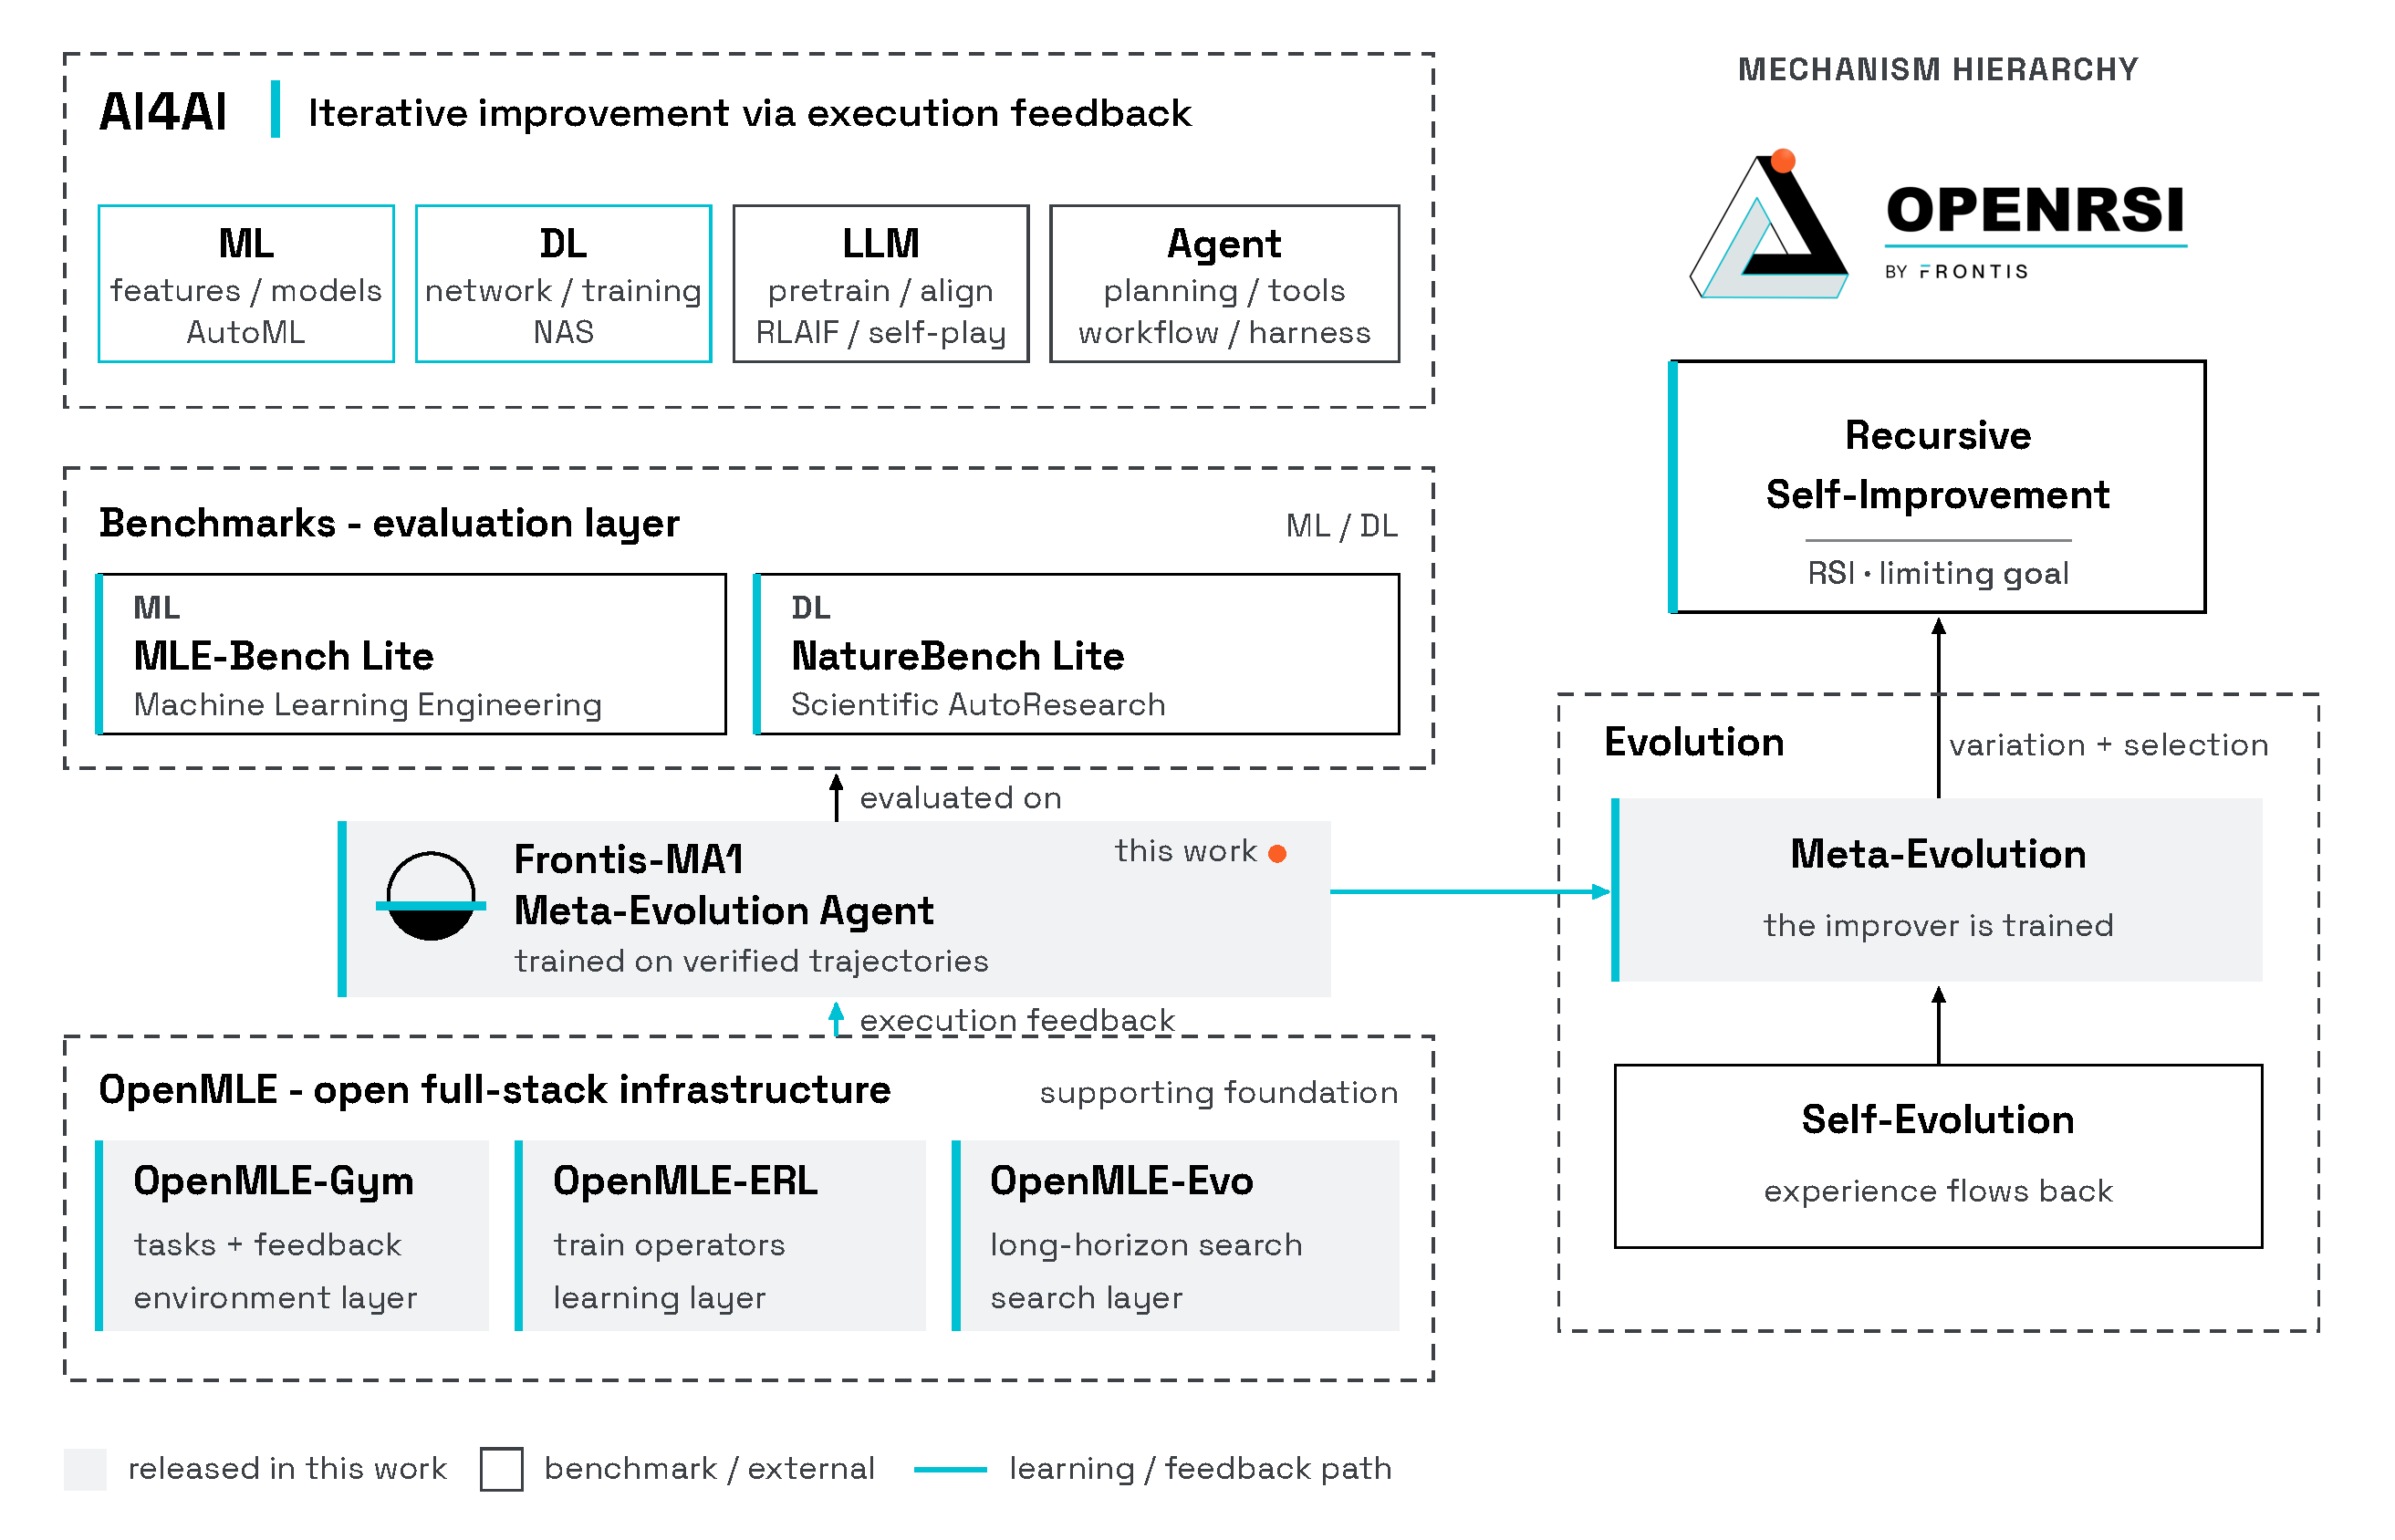
\includegraphics[width=\linewidth]{figures/openmle_positioning_integrated_v3.pdf}
    \caption{Positioning of this work. \textbf{Left:} within AI4AI, machine learning
  engineering (MLE) is our task domain; the OpenMLE stack trains and deploys
  Frontis-MA1, which is both the product of the stack and its engine, evaluated
  only on third-party benchmarks. \textbf{Right:} the mechanism ladder from
  evolution to recursive self-improvement; the meta-evolutionary loop (orange)
  places this work at the level where the improver itself is trained---the level after which Frontis-\textbf{MA}1 (\textbf{M}eta-evolution \textbf{A}gent) is named.}
  \label{fig:positioning}
\end{figure}

Prior work advances MLE agents along three complementary but overlapping strands. The first develops inference-time harnesses based on structured or evolutionary search~\citep{jiang2025aide,fang2025mlzero,nam2025mlestar,du2025automlgen,liu2025ml,zhu2026toward,toledo2025airesearchagents,internscience2026mlevolve}. The second builds executable tasks and environments~\citep{qiang2025mledojo,qiang2025mlesmith,nathani2025mlgym,lupidi2026airs}. The third uses execution feedback to post-train MLE agents~\citep{liu2025mlagent,li2025mlerl,yang2025rlmleagents,cai2026acegrpo}. Some systems bridge subsets of these strands---MLE-Dojo supports model tuning, while AceGRPO recycles iterative execution traces into training~\citep{qiang2025mledojo,cai2026acegrpo}---but, among the representative public systems audited in Appendix Table~\ref{tab:mle-open-release-matrix}, none jointly spans scalable task and environment construction, execution-grounded agent post-training, and an evolutionary harness that deploys the trained agent in long-horizon search, together with the artifacts needed to reproduce the full loop.

We introduce \textbf{OpenMLE}, an open full-stack technical solution for training language models to construct and iteratively improve machine learning solutions using executable feedback: \openmlegym{} constructs 5,758 quality-gated executable tasks and provides isolated execution, structured feedback, and task-specific evaluation; \openmleerl{} uses budget-adaptive supervision fine-tuning and reinforcement learning to turn verified solutions and revisions into stronger MLE behavior; and \openmleevo{} organizes long-horizon search around structured experience, non-greedy selection over quality, progress, and novelty, and operator-conditioned memory. OpenMLE exposes \textsc{Draft}, \textsc{Improve}, \textsc{Debug}, and \textsc{Crossover} as a shared interface between post-training and inference. This interface lets verified evolutionary transitions supervise the same transformations that search later composes, making the trained model the variation engine of the evolutionary harness and forming the meta-evolutionary loop illustrated in Figure~\ref{fig:positioning}, in which the improver itself is trained.
A model trained and deployed in this role is a \textbf{\emph{meta-evolution agent}} as introduced in \citep{jiang2026selfimprovingagents}.



Using OpenMLE, we train \textbf{\thirtyfivebmodel{}}
(\textbf{M}eta-evolution \textbf{A}gent, generation~1) as our primary
model and evaluate it at the model, harness, and system levels on MLE-Bench Lite under a fixed 12 GPU-hour per-task budget. At the model level, under the identical \openmleevo{} harness, \thirtyfivebmodel{} improves over Qwen3.6-35B-A3B from $39.39\%$ to \frontisThirtyFiveEvoResult{} Medal Average and from $0.5828$ to \frontisThirtyFiveEvoHumanRank{} Human Rank. At the harness level, matched comparisons show that \openmleevo{} outperforms general-purpose Claude Code or Codex scaffolds across four frontier models and original AIRA-Evo on \thirtyfivebmodel{}. At the system level, \thirtyfivebmodel{} with \openmleevomax{}\footnote{\openmleevomax{} is an enhanced OpenMLE configuration; see Section~\ref{sec:experimental-setup} for details.} reaches \frontisThirtyFiveEvoMaxResult{} Medal Average and \frontisThirtyFiveEvoMaxHumanRank{} Human Rank, exceeding GPT-5.5 + Codex. As a controlled cross-model replication, \thirtybmodel{} improves over Qwen3-30B-A3B-Thinking-2507 from $34.85\%$ to \frontisThirtyEvoResult{} under the same \openmleevo{} harness. Finally, controlled NatureBench~\citep{wang2026naturebench} Lite comparisons provide evidence that both execution-grounded post-training and adapted evolutionary search transfer beyond competition-style MLE.
We will release the datasets, training and evaluation code, sandbox infrastructure, harness code, and final post-trained checkpoints. This release will make the complete OpenMLE workflow reproducible, enabling broader study of meta-evolution in executable AI4AI settings and its role on the path toward RSI. Our contributions are:
\begin{enumerate}[leftmargin=*,itemsep=2pt,topsep=0pt,partopsep=0pt,parsep=0pt]
\item We present OpenMLE as a full-stack technical solution for studying recursive self-improvement in executable MLE, connecting verifiable environments, post-training, and test-time evolution in one validated workflow.
\item We introduce \openmlegym{}, which unifies 5,758 challenging tasks with isolated execution, structured feedback, and task-specific evaluators for scalable training, search, and evaluation.
\item We introduce \openmleerl{} to train reusable \textsc{Draft}, \textsc{Improve}, \textsc{Debug}, and \textsc{Crossover} operators through execution-grounded supervised fine-tuning and reinforcement learning.
\item We introduce \openmleevo{} to support experience-guided long-horizon search over the environments and feedback exposed by \openmlegym{}.
\item Using the complete stack, we train and release \thirtyfivebmodel{} as our primary model, together with \thirtybmodel{} as a companion model for controlled cross-model replication. Evaluations separate the gains from post-training and search on MLE-Bench Lite and provide transfer evidence on NatureBench Lite. We also release the datasets, training and evaluation code, execution infrastructure, and search framework needed to reproduce and extend OpenMLE.
\end{enumerate}

